%%%%%%%%%%%%%%%%%%%%%%%%%%%%%%%%%%%%%%%%%
% This document provides a sample senior 
% thesis proposal template for use
% by Allegheny's Computer Science majors.
%
% This template was adopted from Jeremie Gillet
% Ref: https://github.com/oist/LaTeX-templates
%
% Author: Janyl Jumadinova
% Last Updated: November 5, 2019
%
%%%%%%%%%%%%%%%%%%%%%%%%%%%%%%%%%%%%%%%%%

%----------------------------------------------------------------------------------------
%	PACKAGES AND OTHER DOCUMENT CONFIGURATIONS
%----------------------------------------------------------------------------------------

\documentclass[12pt,oneside]{book} % 12 pt font, one-sided book style
\usepackage[a4paper, includehead, headheight=0.6cm, inner=3cm ,outer=2.5cm, top=2.5 cm, bottom=2.5cm]{geometry}  % Changing size of document
\usepackage[english]{babel} % The document is in English
\usepackage[utf8]{inputenc} % UTF8 encoding
\usepackage[T1]{fontenc} % Font encoding

\usepackage{graphicx} % For including images
\graphicspath{{./images/}} % Specifies the directory where images are stored

\usepackage{longtable} % tables that can span several pages
\usepackage[bf]{caption} % caption: FIG in bold
\usepackage{fancyhdr} % For the headers

\newcommand{\numberedchapter}{ % Preparation for numbered chapters
	\cleardoublepage % To make sure the previous headers are passed
	\fancyhead[RE]{{\bfseries \leftmark}}% Headers for left pages
	\fancyhead[LO]{{\bfseries \rightmark}}}% Headers for right pages
\newcommand{\unnumberedchapter}[1]{ % Preparation for unnumbered chapters
	\cleardoublepage % To make sure the previous headers are passed
	\addcontentsline{toc}{chapter}{#1} % Also adds the chapter name to the Contents
	\fancyhead[RE]{{\bfseries #1}} % Headers for left pages
	\fancyhead[LO]{}}%Headers for right pages

\usepackage{emptypage} % No headers on an empty page

\usepackage{eso-pic} % For the background picture on the title page
\newcommand\BackgroundPic{%
\put(0,-120){%
\parbox[b][\paperheight]{\paperwidth}{%
\vfill
\centering

\includegraphics[width=4in]{images/logo}%
\vfill
}}}

\usepackage{hyperref} % Adds clickable links at references

%----------------------------------------------------------------------------------------
%	ADD YOUR CUSTOM VALUES, COMMANDS AND PACKAGES
%----------------------------------------------------------------------------------------

% Open preamble/mydefinitions.tex and enter some values (name, thesis title...) 
% and include your own custom LaTeX functions and packages

%----------------------------------------------------------------------------------------
% values for the proposal
%----------------------------------------------------------------------------------------

\newcommand{\name}{Author Name} % Author name
\newcommand{\thesistitle}{Thesis Title} % Title of the thesis
\newcommand{\submissiondate}{\today} % Submission date "Month, date year"
\newcommand{\supervisor}{First Reader} % First reader's name
\newcommand{\cosupervisor}{Second Reader} % Second reader's name


%----------------------------------------------------------------------------------------
%	BIBLIOGRAPHY STYLE 
%----------------------------------------------------------------------------------------


\bibliographystyle{acm}

%----------------------------------------------------------------------------------------
%	YOUR PACKAGES (be careful of package interaction)
%----------------------------------------------------------------------------------------

\usepackage{amsthm,amsmath,amssymb,amsfonts,bbm}% Math symbols

%----------------------------------------------------------------------------------------
%	YOUR DEFINITIONS AND COMMANDS
%----------------------------------------------------------------------------------------

% New Commands
\newcommand{\bea}{\begin{eqnarray}} % Shortcut for equation arrays
\newcommand{\eea}{\end{eqnarray}}
\newcommand{\e}[1]{\times 10^{#1}}  % Powers of 10 notation


\begin{document}

%----------------------------------------------------------------------------------------
%	TITLE PAGE
%----------------------------------------------------------------------------------------

\pagestyle{empty} % No page numbers
\frontmatter % Use roman page numbering style (i, ii, iii, iv...) for the preamble pages

\begin{titlepage}
\AddToShipoutPicture*{\BackgroundPic}
\begin{center}
\vfill
{\large \scshape Allegheny College \\ Department of Computer Science \\ \& \\ Department of Music}\\[1.4cm]
{\Large Senior Thesis}\\[0.5cm]
\rule{\textwidth}{1.5pt}\\[0cm]
{\huge \bfseries \thesistitle \par \ }\\[-0.5cm]
\rule{\textwidth}{1.5pt}\\[2.5cm]
\hfill  by\\[1cm]
\hfill  {\large \bfseries\name}\\
\vfill
{\hfill \large Project Supervisors: \textbf{\supervisor}} \\ 
\ifx\cosupervisor\undefined\else{\hfill \large Co-Supervisors: \textbf{\cosupervisor}} \\ \fi
\vspace{1cm}
\hfill  \submissiondate
\end{center}
\end{titlepage}

\pagestyle{fancy} % Changes the headers
\fancyhf{}% Clears header and footer
\fancyhead[RO,LE]{\thepage} % page number on the outside of headers

%-------------------------------------------------------------------------------
%	PREAMBLE PAGES (delete unnecessary pages)
%   preamble pages besides abstract are optional
%-------------------------------------------------------------------------------

% \unnumberedchapter{Abstract} 
\chapter*{Abstract} 

Provide a concise summary of your  research project of approximately 250 words. 
Remember that the abstract is {\it not\/} an introduction, it is a {\it summary\/} of the entire document, including the results and future direction of the project.
% \unnumberedchapter{Acknowledgments} 
\chapter*{Acknowledgments}
\label{ch:acknowledgements}

\begin{itemize}
	\item Dr. Douglas Jurs and Dr. Janyl Jumadinova for help in designing the research
	\item Dr. James Niblock for help in proofing and editing the manuscript 
\end{itemize}
% \unnumberedchapter{Abbreviations} 
\chapter*{Abbreviations} 

All abbreviations used in the thesis should be listed here, with their definitions, in alphabetical order.  This includes trivial and commonly used abbreviations (at your own discretion), but not words that have entered into general English usage (such as laser or DNA).  In particular, non-standard abbreviations should be presented here.  This is an aid to the reader who may not read all sections of the thesis. \\ % You can delete this paragraph, only the table is needed.

\begin{longtable}{rl}
PPT & positive partial transpose\\
SRPT & Schr\"odinger-Robertson partial transpose
\end{longtable}
% \unnumberedchapter{Glossary} 
\chapter*{Glossary} 

% Break up this table into several ones if it takes up more than one page
\begin{center}
\begin{longtable}{r p{0.58 \textwidth}}
Dipole Blockade & Phenomenon in which the simultaneous excitation of two atoms is inhibited by their dipolar interaction. \\
Cavity Induced Transparency & Phenomenon in which a cavity containing two atoms excited with light at a frequency halfway between the atomic frequencies contains the number of photons an empty cavity would contain.  \\ 
\end{longtable}
\end{center}

% \cleardoublepage
\thispagestyle{empty} % Page style needs to be empty for this page

\vspace*{8cm} 

\hfill
\begin{parbox}{0.6\textwidth}{
	\begin{flushright}
		To Barbara Moore
	\end{flushright}}
\end{parbox}

%-------------------------------------------------------------------------------
%	LIST OF CONTENTS/FIGURES/TABLES
%-------------------------------------------------------------------------------

\unnumberedchapter{Contents}
\tableofcontents % Write out the Table of Contents
\unnumberedchapter{List of Figures}
\listoffigures % Write out the List of Figures
\unnumberedchapter{List of Tables}
\listoftables % Write out the List of Tables

%-------------------------------------------------------------------------------
%	THESIS MAIN TEXT
%-------------------------------------------------------------------------------

\addtocontents{toc}{\vspace{2em}} % Add a gap in the Contents, for aesthetics
\mainmatter % Begin numeric (1,2,3...) page numbering

%\numberedchapter{Introduction} % Title of the numbered chapter
\chapter{Introduction}
\label{ch:intro}

This is the introduction. It should describe your completed senior thesis work, including the overall aims and the background motivating your research. Whenever possible, you should use one or more concrete examples
and technical diagrams. 

It is often useful and necessary to separate the introduction into multiple section. Several possible sections are proposed below, you can use these or distribute your introductory text into sections in another way. 

\section{Motivation} 
\label{sec:motivation}

\section{Current State of the Art}
\label{sec:stateofart}

\section{Goals of the Project}
\label{sec:goals}

\section{Thesis Outline}
\label{sec:outline} % Introduction (first numbered chapter)

%\numberedchapter{Related Work}
\chapter{Related Work} 
\label{ch:relatedwork}

As the field of AI has grown, more and more researchers are looking into the extent of the capabilities of AI.  The creation of music with computers has gained increased attention within the last decade, however, this does not mean that these tools have gained popularity among users.  Quite a few of these composers have been developed, but only a very small number of them have seen industry use and almost none of them have been used outside of research or these niche areas in industry.

\vspace{\baselineskip}

The reason for this primarily is that the focus of researchers when creating these tools is how advanced the composer can be and what new ways can AI be employed to create more original music.  Their focus is not at all on how these tools can be made in a way that they might find a larger user base or even a user base at all.  This limits what might come of these technologies now and in the future.

\vspace{\baselineskip}

Setting this aside, however, the researchers that have developed these composers have created some very impressive tools capable of creating very convincing music.  This project aims more to guide the user through the process of composing music.  This is different than a majority of the research projects in this area that focus on creating a composer that can write its own music, but the writing still contains an important discussion of how computers can be used to create music.

\section{AI Powered Composers}
\label{sec:aipoweredcomposers}

The following works discuss several different AI-based composers that were created to generate their own music.  For the purpose of this thesis, they will be analyzed for their effectiveness at composing as well as their shortcomings as tools that only have limited usability.  All of these have proven to be effective at creating music, but none of them have shown popularity as music composition tools.

\subsection{FlowComposer}
\label{subsec:flowcomposer}

Of the existing AI composers, FlowComposer is the only one that has seen use in industry \cite{Papadopoulos_2016}.  An album that was recorded consisting of only music created with FlowComposer was released in 2017 \cite{Papadopoulos_2016}.  This is also one of the only tools that has an actual visual user interface and is not strictly accessed through the command line.  It is currently being developed as part of Sony CSL and Flow Machines, but is not available to the public for use \cite{Papadopoulos_2016}.  An audio example of what FlowComposer is capable of producing is available on their website, \url{https://www.flow-machines.com}, but access to the tool itself is not provided \cite{Flow_2018}.

\vspace{\baselineskip}

The French composer Jean-Michel Jarre is using Flow Machines to create an "infinite album" \cite{Savage_2019}.  This is a never ending, constantly evolving piece of music generated by Flow Machines from a large library of musical samples \cite{Savage_2019}.  The album is available in JarreLab's EON app \cite{Jarre_2019}.  The music that you hear is generated in real time and will never be heard again \cite{Jarre_2019}.  A link to download the app can be found here: \url{https://jeanmicheljarre.com}.

\vspace{\baselineskip}

FlowComposer was designed to create new songs automatically in any style or can generate the style based on user provided parameters and input \cite{Papadopoulos_2016}.  This tool is capable of re-harmonization (taking an existing melody and create new harmonies in different styles), variation (taking the melody and introducing variations into the pitch content and rhythm), and rendering (playing back a given score as if it were being performed) \cite{Flow_2018}.

\vspace{\baselineskip}

The musical output of this tool is a lead sheet that is scored for a full band.  The music that FlowComposer produces fits into the category of popular songs (e.g. Pop, Jazz, Rock, R \& B, etc.).  It comes out fully notated and able to be performed or recorded.  It is a very high quality tool and very capable at writing songs, but due to its research based nature, is kept from the public.  It is highly likely also that this tool would be very expensive if it were available to the public.  Maybe in the future, this will be a tool that is made available, but it will doubtfully ever be accessible to the average person due to the potential price.

\subsection{BachProp}
\label{subsec:bachprop}

BachProp is a neural composer algorithm that was created to be able to compose new music in any style \cite{Colombo_2018Com}.  It was trained initially on the chorales of J. S. Bach, but is able to compose in any style when given appropriate training data \cite{Colombo_2018Com}.  The data is fed to the composer through MIDI files which are mathematically normalized before being translated into probability data that the algorithm uses to predict melodic direction and shape \cite{Colombo_2018Com}.

\vspace{\baselineskip}

For the evaluation of BachProp, audiences were asked to rate several string quartets that it composed after it was trained on string quartets by Haydn and Mozart \cite{Colombo_2018Com}.  Based on the results of the surveys, the music was not only well received, but it was also quite convincingly in the appropriate style and character \cite{Colombo_2018Com}.  To hear some of the music that Bach Prop composed, visit: \url{https://sites.google.com/view/bachprop-icml18/}.

\vspace{\baselineskip}

The process of actually performing crowd-based musical validation is quite important here.  Rather than the researchers who developed the tool rating the music, they had general audiences perform the reviews to better understand the broad appeal of the music.  In this project, a similar crowd-based reviewing of the interface was performed.  Participants individually judged their created music in their own terms so that their personal success was measured to be able to determine if the user interface was able to guide them through the composition process.

\vspace{\baselineskip}

BachProp has also been used and evaluated in the composition of music in a number of other styles \cite{Colombo_2018Gen}.  The method of musical representation used by BachProp has proven to be more effective at capturing and later translating the information from the provided training scores than other algorithmic composers \cite{Colombo_2018Gen}.  By normalizing how the musical data is stored, this tool is able to gather and retain more detail from the score than other composers \cite{Colombo_2018Gen}.  This is what makes BachProp more effective at emulating a given style and producing more convincing musical output \cite{Colombo_2018Gen}.

\vspace{\baselineskip}

In order for the several Python libraries that were used to create the composer to cooperate, the musical data for this project was also represented in a normalized manner.  Like BachProp, the data was represented as MIDI events to provide a standard for communication and output.  This also means that at any step in the composition process the data could be imported into any standard music notation program and used externally to the composer as MIDI is the standard for digital music notation representation and playback.

\vspace{\baselineskip}

The largest shortcoming of BachProp is that it was not designed in a way that can be used without extensive music or computer science knowledge.  This means that is highly unlikely that it would ever be picked up by someone who simply wanted to play around with it or experiment with it.  There is an extensive setup involved and it cannot be used by any simple means.  However, BachProp is able to produce high quality music in any style and not just popular music as FlowComposer does.

\subsection{DeepBach}
\label{subsec:deepbach}

DeepBach is a graphical model for musical composition that is designed to be effective at producing polyphonic music in four-part hymn format \cite{Hadjeres_2016}.  This is yet another composer that was trained on the music of J. S. Bach in order to teach it the mechanics of composition and in this case, to teach it chorales specifically \cite{Hadjeres_2016}.  This composer is able to produce convincing Bach chorale style pieces that are driven by user parameters and input \cite{Hadjeres_2016}.  The following are examples of chorales composed by DeepBach.  Below each, is a chordal analysis in slash chord notation.

\pagebreak

It is important to note that examples (a) and (b) were created using the same user input data and parameters.  This shows that there are at least several different possibilities for harmonization and development of the melodic line.  Before the individual examples are discussed, there are some important similarities that are shared between the chorales.

\vspace{\baselineskip}

The first of these is the handling of steps and leaps in each of the voices.  It will later be discussed that it is appropriate to move in step wise motion in the opposite direction after leaping.  In each voice of the voice parts in the examples, this rule is exactly followed.

\vspace{\baselineskip}

The next similarity is in the cadences at the ends of the chorales.  In both example (a) and (c) we see, in the last three chords, a move from some version of V7 of V, to V, to I.  This is a very typical progression and is resolved correctly in both the soprano and bass voices by stepping and leaping respectively.  In example (b) we have a similar progression, but it does not use V7 of V.

\vspace{\baselineskip}

Another similarity comes in the treatment of the different voices.  The soprano voice, which has the melody, contains much less motion and overall activity as compared to the other voices.  This is good practice in melody composition as the melody should be easy to remember and sing back.

\vspace{\baselineskip}

Yet another similarity can be found with the use of chromaticism in the passing tones and shift between chords.  To provide both harmonic interest and a form of melodic interest within each of the parts, some chromatic motion is used.  When it is used, it is resolved appropriately with stepwise motion.

\pagebreak

\begin{figure}[!htbp]
	\centering
	\caption{Score (a) from Hadjeres's published paper showing DeepBach output \cite{Hadjeres_2016}}
	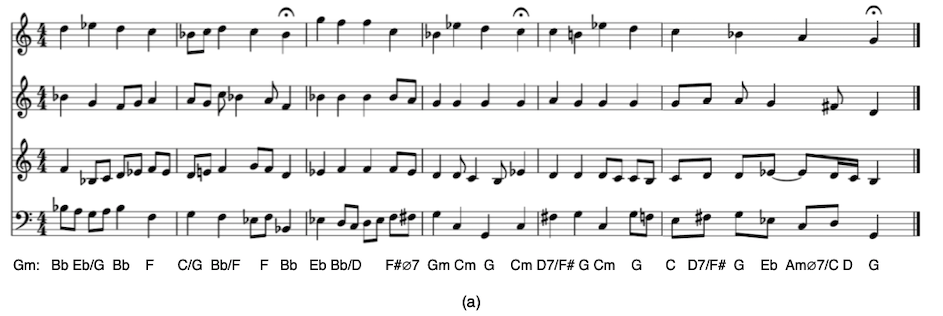
\includegraphics[scale=0.3]{images/deepbachOutputA.png}
\end{figure}

This example (a) is in the key of G Minor.  While it does end in G Major, the presence of B\fl 's and E\fl 's put it in G Minor.  The fact that it ends in G Major is not uncommon however.  It was often the practice to end a chorale in a minor key with the major version of the I chord by raising the third.

\vspace{\baselineskip}

This example in particular uses more chords outside of the normal key material than the other two.  However, the two cadences within the chorale (indicated by the fermatas) are both firmly within G Minor.

\begin{figure}[!htbp]
	\centering
	\caption{Score (b) from Hadjeres's published paper showing DeepBach output \cite{Hadjeres_2016}}
	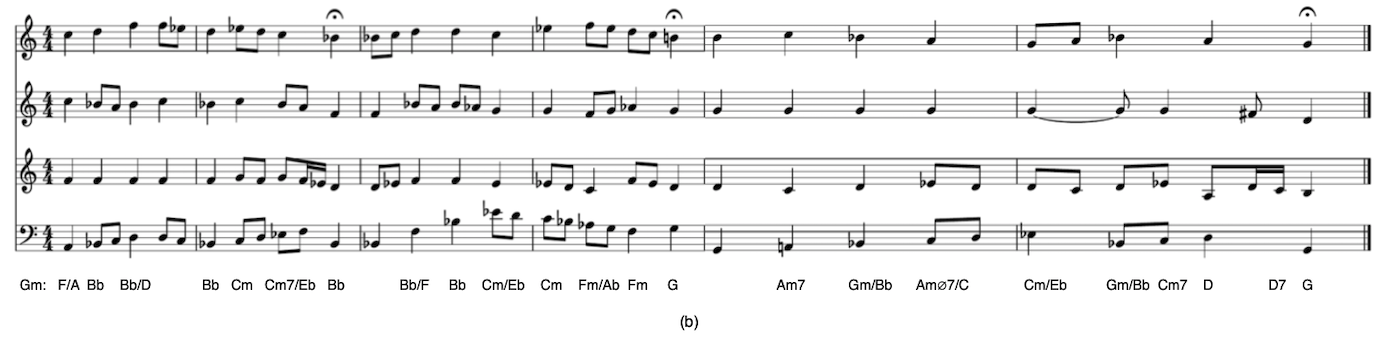
\includegraphics[scale=0.3]{images/deepbachOutputB.png}
\end{figure}

As mentioned previously, this example (b) was made with the same user input data as the previous example.  Also like the first example, this one also ends in the parallel major.  This is not a requirement of this style.  Both examples just happen to leverage this technique.

\vspace{\baselineskip}

This example has some out of key material, but not as much as the first example.  It also moves to the relative major in the second of the two internal cadences instead of only at the end.  While they do share the same metadata, they are distinct in their melodies, progressions, and voice leading.

\pagebreak

\begin{figure}[!htbp]
	\centering
	\caption{Score (c) from Hadjeres's published paper showing DeepBach output \cite{Hadjeres_2016}}
	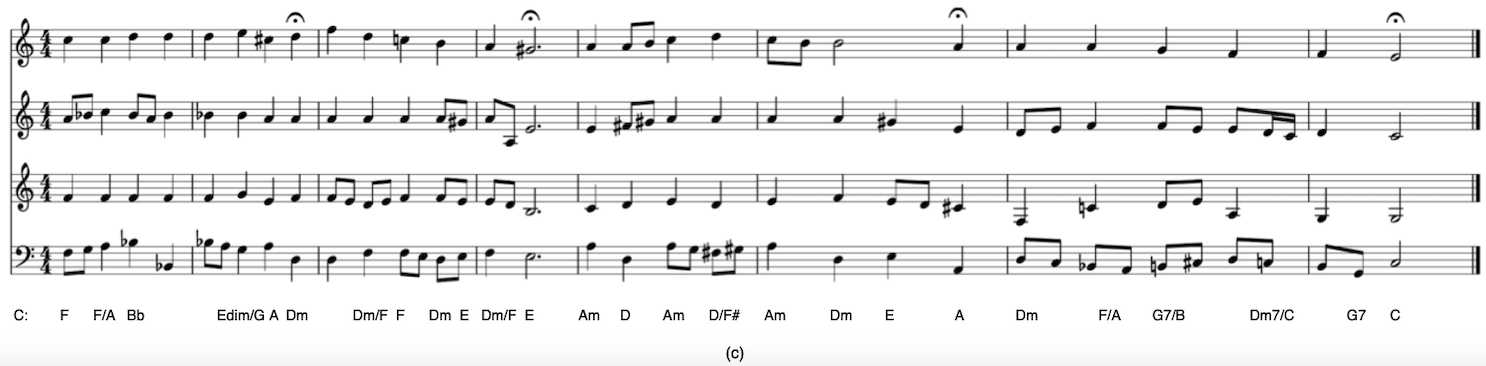
\includegraphics[scale=0.3]{images/deepbachOutputC.png}
\end{figure}

This third example (c) is in C Major.  It also has one more cadence than the other two examples.  Another factor that makes this example different is that there is noticeably more chromatic motion in each of the voice parts.

\vspace{\baselineskip}

While this has more material from outside the key than the second example, it does not have as much as the first.  In this case however, the internal cadences are from outside the key.  They are, however, distantly related as E Major is V of A Major, A Major is V of D Minor, D Minor is V of G Major, and G Major is V of C Major.  This progression can be seen across the chords at the second two fermatas and final three chords.

\vspace{\baselineskip}

DeepBach does provide integration with the notation program MuseScore \cite{Hadjeres_2016}.  This means that there is a way in which people who are familiar with notation software could use this composer.  While this is better than many of the others, it still requires a fair bit of prior knowledge.  Additionally, this composer is not capable of operating in more than four-part chorale style.  The potential uses of this composer are very limited due to this fact.

%\numberedchapter{Method Of Approach}
\chapter{Method of Approach} 
\label{ch:method}

This section has been broken down into three parts that each detail a different segment of the project that was completed.  The first section describes the process and tools needed to develop the composer, the second section describes the process and ideas behind the development of the user interface, and the third section describes how the user interface study was designed and conducted.

\section{Computer Composer Development}
\label{sec:composerdev}

While having the functioning composer is an integral part of this project, the most important work here was done on the development of the user interface as this is where other composers in the past have been lacking.  This being said, rather than building the composer from scratch, several Python tools and libraries were employed to created the backend of the tool.

\vspace{\baselineskip}

None of these tools on their own were capable of forming the functioning composer.  Several of them have very advanced sets of functions, but these were not all of what was required to build the composer.  To complete the tool for this project, the output of each of these libraries was normalized and then transferred from one to another to reach the final output.  The following table lists all of the tools that were used and their specific functions within the composer.

\begin{table}[]
	\centering
	\caption{Python tools and libraries and their uses in this project}
	\begin{tabular}{|l|l|}
		\hline
		music21 & Melody Generation, Harmonization \\ \hline
		MIDI Miner & Tonal Analysis, Key Analysis, Mood Analysis \\ \hline
		MIDI Musical Accompaniment & Accompaniment Generation \\ \hline
		Kodou & Notation \\ \hline
		mingus & Interface Link \\ \hline
		LilyPond & Notation Output \\ \hline
		Improviser & Part Generation \\ \hline
	\end{tabular}
\end{table}

\subsection{Main Composer Functions}
\label{composerfunctions}

There are several important functions that any of these computer composers should have.  This includes: melody generation, harmonization, key and metric analysis, orchestration, and notation.  The following chart demonstrates the process taken to compose using this tool.

\begin{figure}[h!]
	\centering
	\caption{Composition process flowchart}
	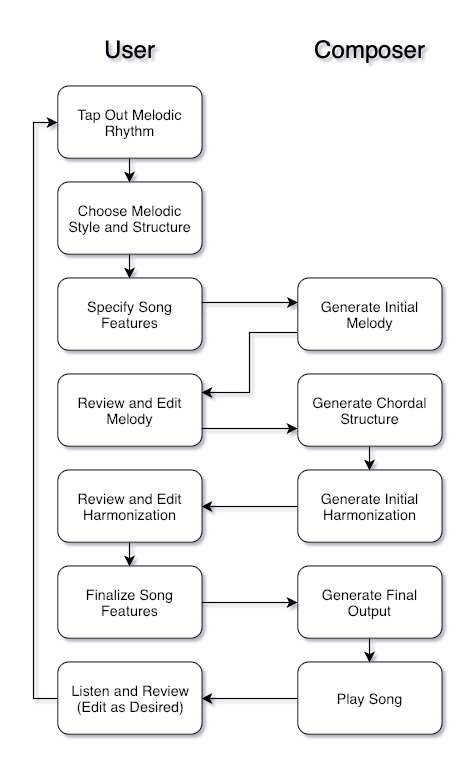
\includegraphics[scale=0.7]{images/composerProcess.png}
\end{figure}

\pagebreak

\subsubsection{Melody Generation}
\label{subsubsec:melody}

During this initial part of the composition process, the computer assists the user in creating a "good" melody.  This involves determining the contour, rhythm, conjunction and disjunctions, and pitches of the melody.  After the melody is generated, the computer determines if it is able to harmonize the melody.  If it is not, it goes back and guide the user through the problematic areas.

\vspace{\baselineskip}

The user also has the opportunity to change the melody if they do not like the way that it sounds or are not satisfied with what they have created.  The computer also provides tips on how to make better melodies and makes suggestions based on the melody that has been generated.

\subsubsection{Harmonization}
\label{subsubsec:harmony}

Next, the computer takes the melody that it has determined that it can harmonize and performs an initial harmonization.  By default, this follows the standard progression of chords in western music as displayed below.

\begin{figure}[h!]
	\centering
	\caption{Standard major key harmonic progression}
	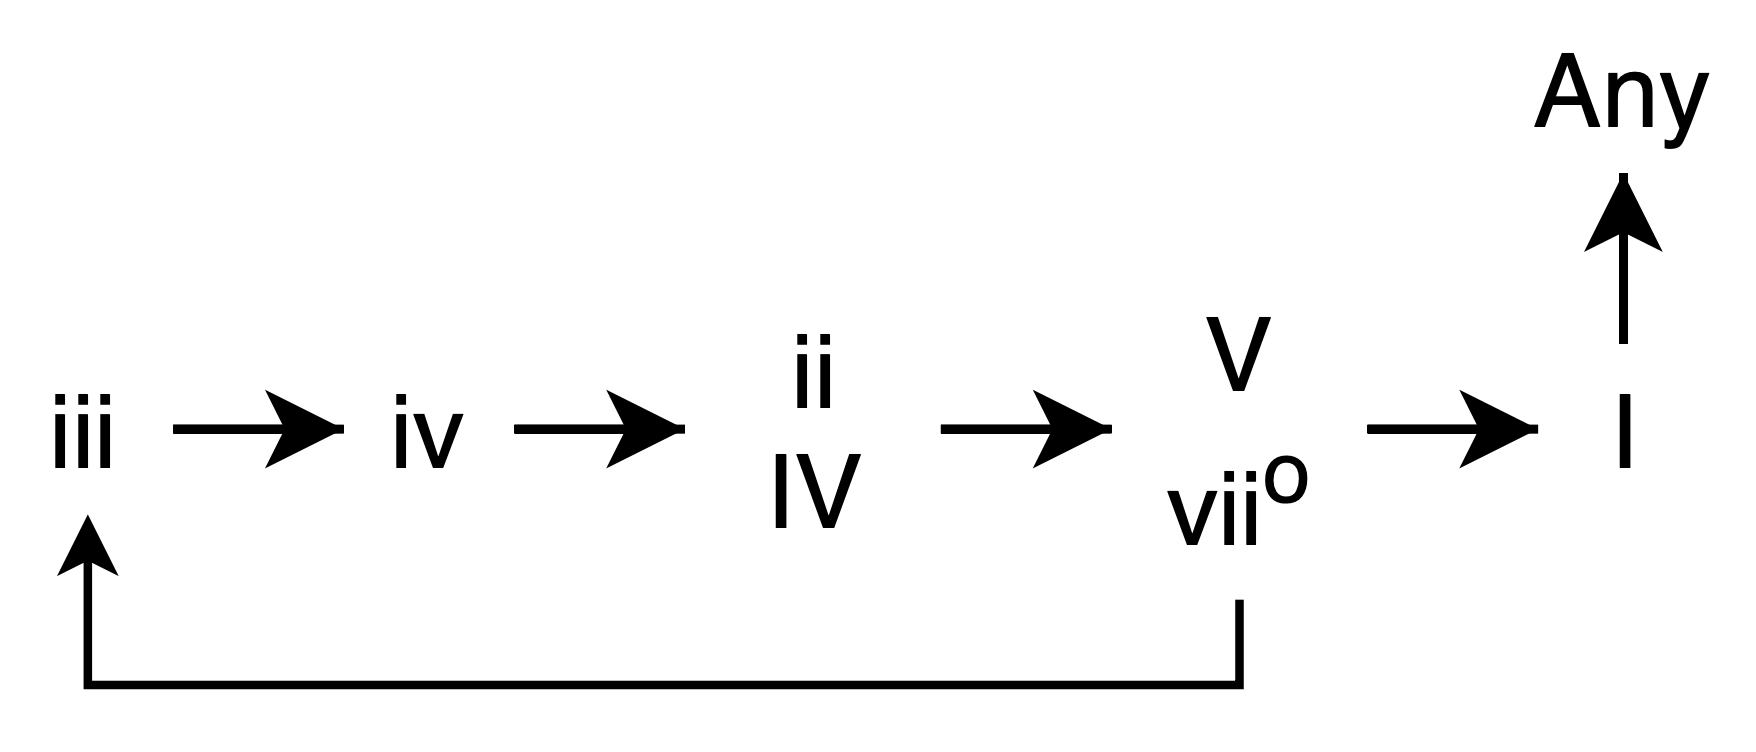
\includegraphics[scale=0.25]{images/majorProgression.png}
\end{figure}

\begin{figure}[h!]
	\centering
	\caption{Standard minor key harmonic progression}
	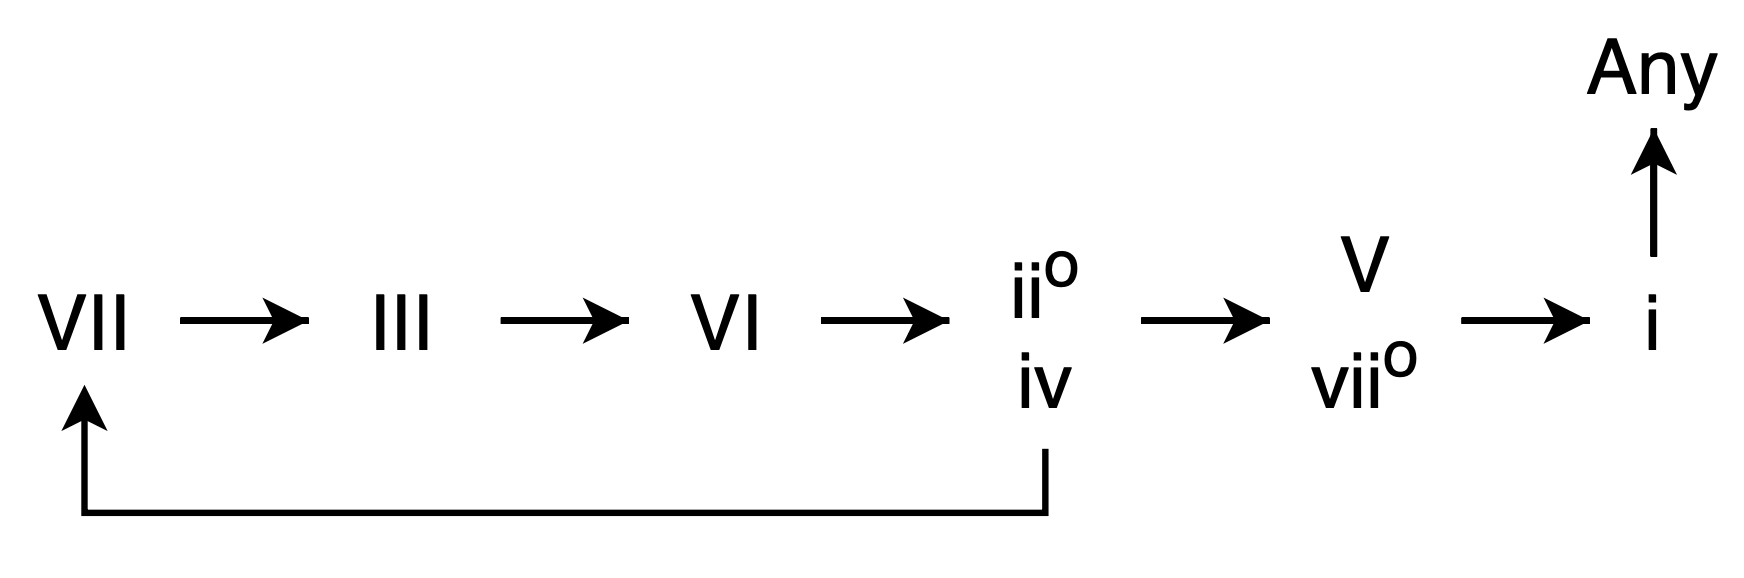
\includegraphics[scale=0.33]{images/minorProgression.png}
\end{figure}

The user is presented with a listing of the chords created during the harmonization and has a change to hear the progression and choose an alternative chord that still fits the melody.  The user also has the option to create their own progression without the rules of western progression in place.

\subsubsection{Key and Metric Analysis}
\label{subsubsec:analysis}

The next step in the composition process metric and key analysis of the melody and harmony that were previously generated.  This step is important for adding additional parts during orchestration and the final notation step.  For the purpose of sound to the user, this does not matter, but it is require to be able to notate the composition.

\vspace{\baselineskip}

This step also contains mood analysis for the purpose of providing the user with an idea of how what they are composing might feel.  This provides them with a general affect of the piece and gives them some information as to what sound set of instruments to pick from.

\subsubsection{Orchestration}
\label{subsubsec:orchestration}

\subsubsection{Notation}
\label{subsubsec:notation}

\subsection{Tools}
\label{subsec:tools}

The following is a descriptive list of the tools that were used in the creation of this composer.

\begin{itemize}
	\item MIDI Miner
	\begin{itemize}
		\item This is a Python library that is capable of analyzing music's tonal tension and classifying parts into different musical segments.  This is used in the composition process to determine the mood and structure of the musical output.
	\end{itemize}
	\item MIDI Musical Accompaniment
	\begin{itemize}
		\item This is a tool, written in Python, that creates musical accompaniment after being provided with instructions in a text file.  This tool is used to generate additional parts automatically based on the lines that the user creates.  The instruction file is be populated by user choices such as style and tempo and by the composer's analysis with details such as key and structure.
	\end{itemize}
	\item Kodou
	\begin{itemize}
		\item Kodou is a Python package that does algorithmic music notation.  This was helpful to be able to take the music created by the tool and output it to a file in standard music notation so that it can be taken and read by another musician.
	\end{itemize}
	\item mingus
	\begin{itemize}
		\item This is a tool that is capable of a number of useful functions for this composer.  Generally, it is a music theory and notation package for Python, but more specifically, it can help build editors, educational music theory tools, and other music processing applications.
	\end{itemize}
	\item LilyPond
	\begin{itemize}
		\item LilyPond Is a program that can interface with a Python program in order to output music notation files.  Kodou and mingus both use LilyPond for their notation output functions.
	\end{itemize}
	\item music21
	\begin{itemize}
		\item This is a set of tools that was developed by MIT for music theory, music computation, and generative composition.  music21 contains the central set of functions that power the composer.
	\end{itemize}
	\item Improviser
	\begin{itemize}
		\item This is Python based software that was created to perform real-time music generation.  Improviser is used in conjunction with music21 to perform the bulk of the back-end work when generating the compositions.
	\end{itemize}
\end{itemize}

%\numberedchapter{Experimental Results}
\chapter{Experimental Results} 
\label{ch:experimentalresults}

To evaluate the success of the composer, it seemed most appropriate to have a user experience study.  It would not be a fair test of how effective the tool is at helping a person compose if the only people that were to test the tool have high level music and computer science knowledge.  To truly understand how the tool performs, it needed to be placed in the hands of a general audience.

\vspace{\baselineskip}

When designing software, two of the key elements are the user interface (UI) and user experience (UX).  The UX is how the user feels about and responds to a product.  It is based on how the tool is presented, acquired, and how it functions.  This chapter of the document details the design of the UX study, its evaluation, and any potential threats to its validity.

\section{User Experience Study}
\label{sec:userexperiencestudy}

As a part of this study, there are several important metrics that had to be gauged in order to determine the effectiveness of the tool.  These include:

\begin{itemize}
	\item User Background
	\item System Availability
	\item System Performance
	\item System Accessibility
	\item User Impressions
\end{itemize}

Several questions were presented to the user about specific areas within each of these larger categories.  This data was then used to determine the performance in the category as a whole.  The specific categories, subcategories, and related questions are listed below.

\subsection{User Background}
\label{subsec:userbackground}

This sections asks the user some demographic questions related to the user's previous experience and gets important connecting information.

\subsubsection{Music Background}
\label{subsubsec:musicbackground}

Rate your amount of music theory knowledge.

\begin{itemize}
	\item No Knowledge
	\item Beginner
	\item Intermediate
	\item Advanced
	\item Expert
\end{itemize}

\noindent Rate your ability to read music.

\begin{itemize}
	\item No Knowledge
	\item Beginner
	\item Intermediate
	\item Advanced
	\item Expert
\end{itemize}

\noindent Rate your knowledge related to instrumental and/or vocal performance.

\begin{itemize}
	\item No Knowledge
	\item Beginner
	\item Intermediate
	\item Advanced
	\item Expert
\end{itemize}

\noindent Have you had musical instruction?

\begin{itemize}
	\item Yes
	\item No
\end{itemize}

\noindent If yes, please select all of the following types that apply.

\begin{itemize}
	\item Instrumental Instruction
	\item Vocal Instruction
	\item Theory Instruction
	\item History Instruction
	\item Composition Instruction
\end{itemize}

\noindent Have you written/composed music in the past?

\begin{itemize}
	\item Yes
	\item No
\end{itemize}

\subsubsection{Computer Science Background}
\label{subsubsec:computersciencebackground}

Rate your amount of computer science knowledge.

\begin{itemize}
	\item No Knowledge
	\item Beginner
	\item Intermediate
	\item Advanced
	\item Expert
\end{itemize}

\noindent Have you had some form of computer science instruction?

\begin{itemize}
	\item Yes
	\item No
\end{itemize}

\noindent If yes, please select all of the following types that apply.

\begin{itemize}
	\item Self Taught
	\item Online Instruction
	\item Classroom Instruction
	\item Professional Instruction
\end{itemize}

\subsubsection{Composition Analysis}
\label{subsubsec:compositionanalysis}

Would you like to submit your compositions for analysis?

\begin{itemize}
	\item Yes
	\item No
\end{itemize}

\noindent If yes, would you like to be listed as the composer?

\begin{itemize}
	\item Yes
	\item No
\end{itemize}

\noindent If yes, please provide how you wish to be named.

\subsection{System Availability}
\label{subsec:systemavailability}

This particular metric deals with whether or not the user was able to access the site and on what sort of device and conditions they had when the attempted to access the site.

\subsubsection{General Access}
\label{subsubsec:generalaccess}

Were you able to access and use the site?

\begin{itemize}
	\item Yes
	\item No
\end{itemize}

\vspace{\baselineskip}

\noindent Did you try on more than one occasion?

\begin{itemize}
	\item Yes
	\item No
\end{itemize}

\subsubsection{Platform}
\label{subsubsec:platform}

On what sort of device did you try to use the site?

\begin{itemize}
	\item Desktop Computer
	\item Laptop
	\item Tablet
	\item Mobile Phone
	\item Other
\end{itemize}

\subsubsection{Operating System}
\label{subsubsec:operatingsystem}

What operating system do you have on your device?

\begin{itemize}
	\item Windows
	\item macOS
	\item iOS
	\item Linux
	\item Android
	\item Other
\end{itemize}

\subsubsection{Browser}
\label{subsubsec:browser}

What web browser were you using?

\begin{itemize}
	\item Chrome
	\item Safari
	\item Internet Explorer
	\item Microsoft Edge
	\item Firefox
	\item Other
\end{itemize}

\subsection{System Performance}
\label{subsec:systemperformance}

This metric deals with how quickly and completely the system responded to the user.

\subsubsection{Load Time}
\label{subsubsec:loadtime}

Did each of the pages load quickly?

\begin{itemize}
	\item Yes
	\item No
\end{itemize}

\noindent If no, with which page(s) did the issue occur?

\subsubsection{Analysis Speed}
\label{subsubsec:analysisspeed}

Were the analysis, notation, and playback returned quickly?

\begin{itemize}
	\item Yes
	\item No
\end{itemize}

\subsubsection{Rendering Issues}
\label{subsubsec:renderingissues}

Was there any part of the page that was missing?

\begin{itemize}
	\item Yes
	\item No
\end{itemize}

\noindent If yes, with which page(s) did the issue occur?

\subsection{System Accessibility}
\label{subsec:systemaccessibility}

This metric deals with the elements of the UI.

\subsubsection{Layout}
\label{subsubsec:layout}

Does the layout of the pages make sense to you?

\begin{itemize}
	\item Yes
	\item No
\end{itemize}

\noindent If no, with which element(s) did you have an issue?

\subsubsection{Design}
\label{subsubsec:design}

Does the overall design of the page and the elements make sense to you?

\begin{itemize}
	\item Yes
	\item No
\end{itemize}

\noindent If no, which which item(s) did you have an issue?

\subsubsection{Sizing}
\label{subsubsec:Sizing}

Was everything on the page sized appropriately to make it easy to use?

\begin{itemize}
	\item Yes
	\item No
\end{itemize}

\noindent If no, which which element(s) did you have an issue?

\subsection{User Impressions}
\label{subsec:userimpressions}

This sections determines the user's progress though the tool and their overall comments about using it.

\subsubsection{Completion}
\label{subsubsec:completion}

Were you able to go through the entire composition process?

\begin{itemize}
	\item Yes
	\item No
\end{itemize}

\noindent If no, where did you stop?

\noindent Why did you stop?

\subsubsection{Frustrations}
\label{subsubsec:Frustrations}

Was there any part of using this tool that was frustrating or upsetting?

\begin{itemize}
	\item Yes
	\item No
\end{itemize}

\noindent If yes, with what part(s) of the tool did you experience this with?

\subsubsection{Changes}
\label{subsubsec:Changes}

Are there any changes that you would make to this tool?

\begin{itemize}
	\item Yes
	\item No
\end{itemize}

\noindent If yes, what are they?

\subsubsection{Comments}
\label{subsubsec:Comments}

What other comments do you have for the developer of this tool?

\section{Study Evaluation}
\label{sec:studyevaluation}



\section{Threats to Validity}
\label{sec:threatstovalidity}



%\numberedchapter{Conclusion}
\chapter{Discussion and Future Work}  
\label{ch:conclusion}

This is the conclusion. You might want to leave it unnumbered, as it is now. If you want to number it, treat it like any other chapter.

This chapter usually contains the following items, although not
necessarily in this order or sectioned this way in particular.

\section{Summary of Results}
A discussion of the significance of the results
and a review of claims and contributions.

\section{Future Work}

\section{Conclusion}


%----------------------------------------------------------------------------------------
%	BIBLIOGRAPHY
%----------------------------------------------------------------------------------------

\addtocontents{toc}{\vspace{2em}} % Add a gap in the Contents, for aesthetics
\unnumberedchapter{Bibliography} % Title of the unnumbered chapter
\bibliography{preamble/bibliography} % The references information are stored in the file named "bibliography.bib"

\end{document}  